\documentclass[UTF8]{ctexart}
\usepackage{amsmath, amssymb}  % fundamental math packages
% American Math Society math and symbol 
\usepackage{tikz}    % Use the package of the MikTex(Then the package of Miktex will be used)
\usepackage{geometry}   % use the packages ---> the most fundamental package is the geometry package  (don't care about the not found since it actually works)  --> if new package are needed, we can use Miktex consol to install it.
\usepackage{graphicx}   % embed *.jpg pictures and *.png pictures
\usepackage{ulem}   % this is for using the uuline and uwave
\usepackage{array}	
\usepackage{verbatim}

\begin{document}
	\Huge
	\begin{center}
		
		\begin{figure}
			\centering
			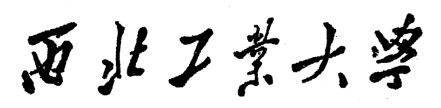
\includegraphics[width=0.9\linewidth]{img/NPU_font}
			\caption{}
			\label{fig:npufont}
		\end{figure}
		
	\end{center}
\end{document}
